
\section{Introduction}
The Risk Modeller's Toolkit (or RMTK) is a Python 2.7 library of functions written by scientists at the GEM Model Facility, which is intended to provide scientists and engineers with the tools to help create the vulnerability input models that go into the OpenQuake risk engine. The intention of this software is to provide scientists and engineers with the means to apply some of the most commonly used algorithms for preparing vulnerability models using structural analysis data. The current approach consists of the derivation of fragility curves and the combination with a damage-to-loss function for the definition of a discrete vulnerability function. The just released GEM analytical vulnerability guidelines have been integrated in this tool and some of the methodologies indicated have been already implemented in the library. In forthcoming versions will hope to make available more methodologies for the process indicated here, and to integrate new functionalities for i) building structural models of different levels of complexity within the RMTK in combination with a structural analysis software, ii) running dynamic and static analysis within the RMTK in combination with a structural analysis software, iii) deriving vulnerability curves directly applying engineering demand parameters-to-loss functions to structural analysis results.

This section provides a description of the methods currently implemented in the RMTK, and an initial presentation of the input and output files is provided. In the following sections, the contents and structure of these files are discussed in detail.

\section{Getting Started and Running the Software}
Install notebook and dependencies. go to folder in the command line (RMTK/Vulnerability/name-of-the-procedure)
 
\section{Nonlinear Static Method with dispersion information}
Nonlinear Static Methods are based on the use of capacity curves resulting from nonlinear static pushover analysis to determine the median seismic intensity values $\hat{s}_c$ corresponding to the attainment of a certain damage state threshold (limit state) and the corresponding dispersion $\beta_{sc}$. These parameters are used to represent a fragility curve as the probability of the limit state capacity C being exceeded by the demand D, both expressed in terms of intensity levels (s$_c$ and s respectively), as shown in the following equation:

\begin{equation}
P_{LS}(s) = P(C < D | s) = \Phi(\frac{ln s -ln \hat{s}_c}{\beta_{sc}})
\end{equation}

The methodology implemented so far in the RMTK allows to consider different shapes of the pushover curve, multilinear and bilinear, record-to-record dispersion and dispersion in the damage state thresholds. Different input types can be inserted depending on whether the user has already at his disposal an idealised pushover curve or it has to be derived from the raw results of a pushover analysis. The intensity measure to be used is S$_a$ and a mapping between any engineering demand parameter (EDP), assumed to describe the damage state thresholds, and the roof displacement is available from the pushover analysis.

Ruiz-Garcia and Miranda (2007) study on inelastic displacement demand estimation, and Vamvatsikos and Cornell (2006) work on seismic demand estimation with multilinear static pushover curves, have been integrated in two nonlinear static procedures within the same script, to give the user the chance to select the procedure with the degree of accuracy consistent with the input available and the structural analyses performed. In the following sections the workflow and the two procedures are presented, following the steps of their implementation in the python script and the necessary scientific background behind it.

\subsection{Method Workflow}
To get started with the Nonlinear Static Method a command line text editor should be used to enter manually the folder location where the RMTK has been saved. The user should add the path \textit{/RMTK/Vulnerability/NSP}, where the Nonlinear Static Method with dispersion information script (\textit{NSM\_dispersion.py}) is located, as shown in the example below:

\begin{Verbatim}[frame=single, commandchars=\\\{\}, samepage=true]
\$ cd path/to/rmtk/folder/RMTK/Vulnerability/NSP
\end{Verbatim}

From the text editor iPython browser page can be opened with the following command line:

\begin{Verbatim}[frame=single, commandchars=\\\{\}, samepage=true]
\$ ipython-2.7 notebook --pylab=inline
\end{Verbatim}

Once the iPython page is opened on the browser, the python scripts contained in the NSP directory will be visible (Figure \ref{fig:notebook}). The file \textit{NSM\_dispersion.ipynb} should be selected to start the calculations.

\begin{figure}[H]
\centering
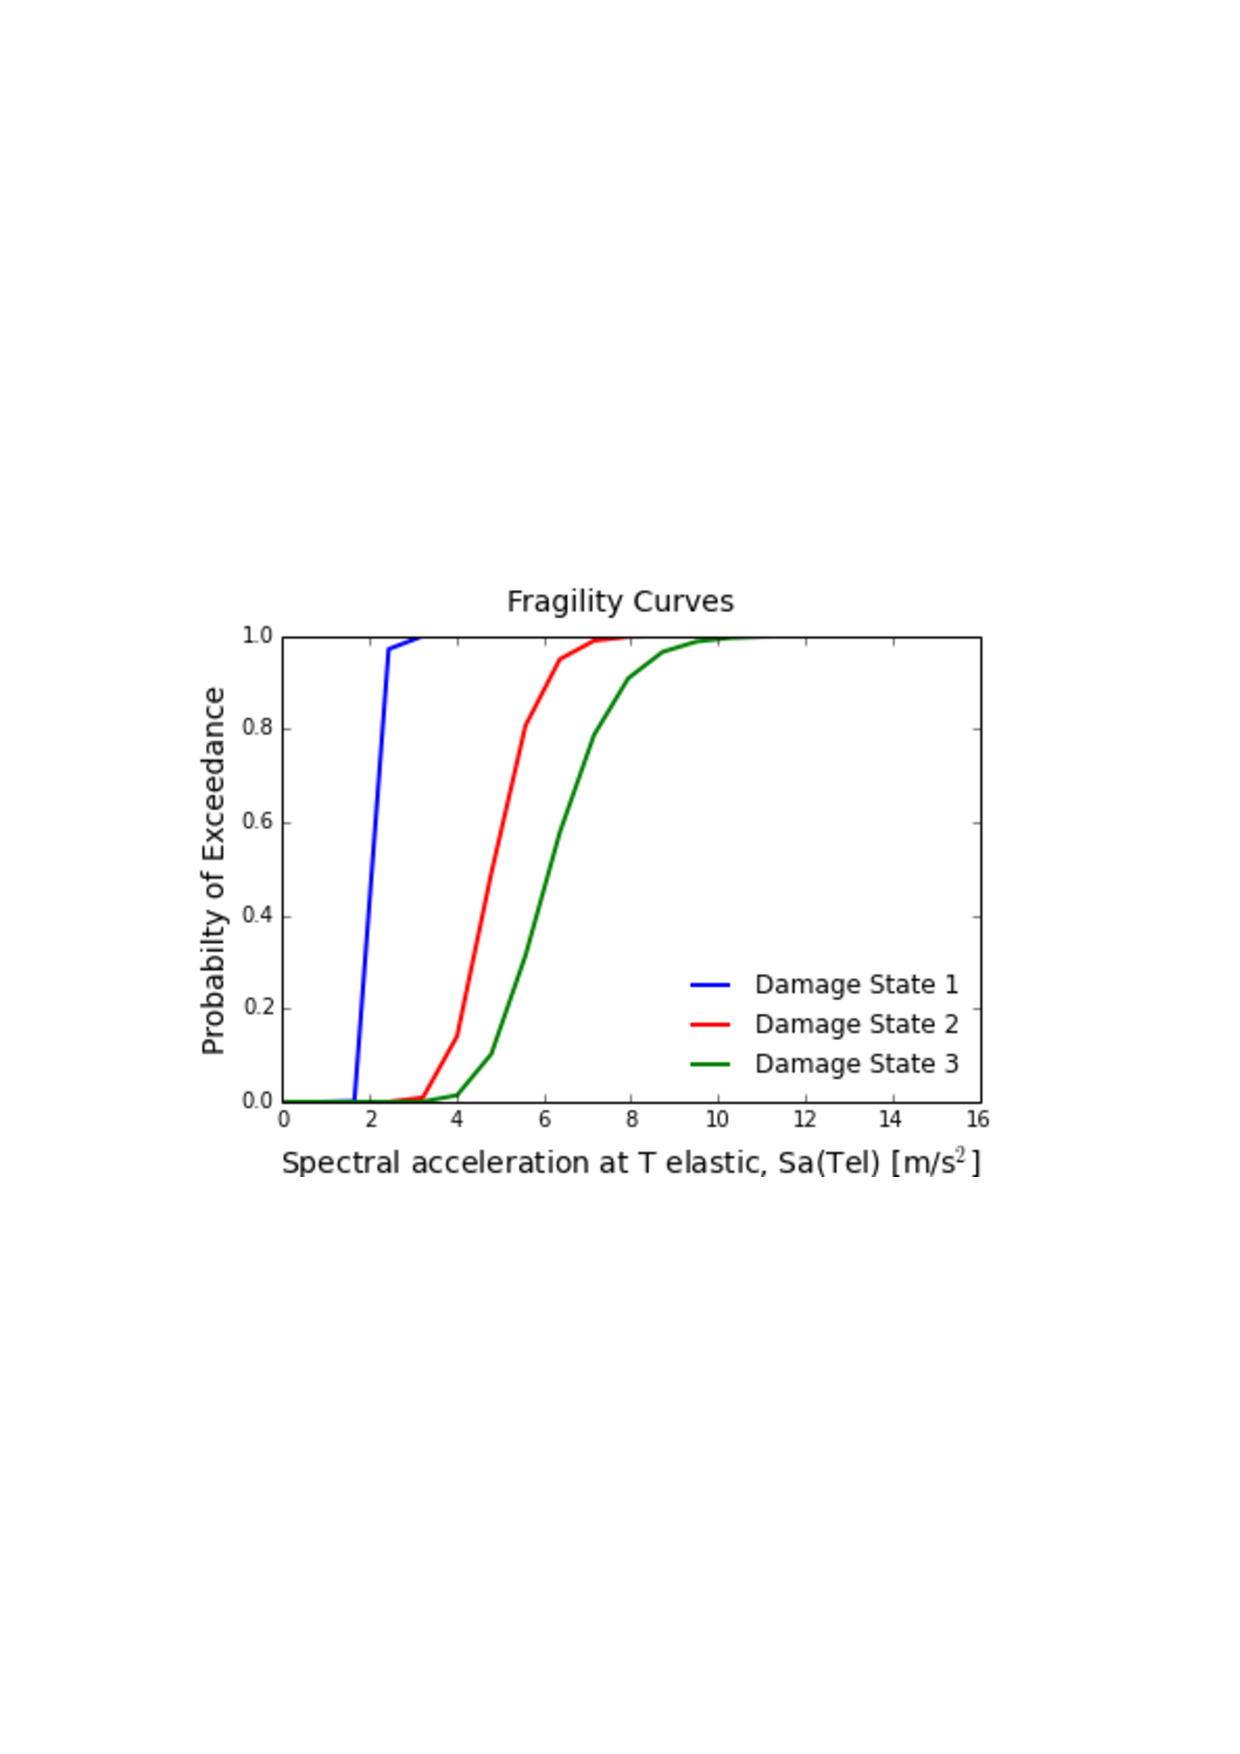
\includegraphics[width=12cm,height=8cm]{./figures/IdealisedCurve.pdf}
\caption{iPython Notebook}
\label{fig:notebook}
\end{figure}

In the first step of the code the initial options and the inputs must be defined, as described in the following section. 

\subsubsection{Options}
\label{par:options}
In the Options the user has to define first of all the type of procedure to be performed and the type of inputs at disposal, setting the variables \textit{an\_type} and \textit{in\_type} respectively. With the variable \textit{an\_type} he can choose between:

\begin{Verbatim}[frame=single, commandchars=\\\{\}, samepage=true]
an\_type = 0 # Cr based procedure (Ruiz-Garcia and Miranda, 2007)
an\_type = 1 # spo2ida procedure (Vamvatsikos and Cornell, 2005)
\end{Verbatim}

With the variable \textit{in\_type} the user can choose between:

\begin{Verbatim}[frame=single, commandchars=\\\{\}, samepage=true]
in\_type = 0 # idealised pushover curve
in\_type = 1 # raw results from a pushover analysis
\end{Verbatim}

The variable vulnerability instead gives the opportunity to stop the process at the derivation of the fragility curves, or to go all the way up to the vulnerability curve definition applying damage-to-loss functions.

\begin{Verbatim}[frame=single, commandchars=\\\{\}, samepage=true]
vulnerability = 0 # stop at fragility curves 
vulnerability = 1 # derive vulnerability curve
\end{Verbatim}

The variable \textit{g} serves the purpose of defining the units that are being used. A floating number must be assigned to the gravity acceleration, compatible with the units used for the period of vibration and for the displacements (if the period is expressed in seconds and displacements are in meters, then g = 9.81). The variable \textit{iml} is a numpy array that identifies the intensity measure levels for which loss ratios are computed and provided in the vulnerability curve.

\begin{Verbatim}[frame=single, commandchars=\\\{\}, samepage=true]
g = 9.81
iml = np.linspace(0.1,15,100)
\end{Verbatim}

The variable \textit{plotflag} allows or inhibits the displaying of plots. It is a list composed of 4 integers, each one controlling a different plot: idealised pushover curve, 16\%-50\%-84\% ida curves, fragility curves, vulnerability curve. Each integer can take as value either zero or one, whether the corresponding graph has to be displayed or not:

\begin{Verbatim}[frame=single, commandchars=\\\{\}, samepage=true]
plotflag = [1, 1, 1, 1] # plot all the graphs
plotflag = [0, 0, 0, 0] # do not plot any graph
\end{Verbatim}

The following variables set some of the characteristics of the plots:

\begin{itemize}
\item \textit{linew}: integer for defining lines width.
\item \textit{fontsize}: fontsize used for labels, graphs etc.
\item \textit{units}: list of 3 strings defining displacements, forces and Spectral acceleration units, as ['[kN]', '[m]', '[m/s$^2$]'], to be displayed on the axes of the plots.
\end{itemize}

The last set of variables is needed for spo2ida procedure only:

\begin{itemize}
\item \textit{pw}: floating number assigning pinching level (from 0 to 1)
\item \textit{filletstyle}: integer enabling or not the use of a spline line to link branches of IDA curves

\begin{Verbatim}[frame=single, commandchars=\\\{\}, samepage=true]
filletstyle = 0 # don't use spline curve
filletstyle = 3 # use spline (recommended)
\end{Verbatim}

\item \textit{N}: number of points per segment of IDA curve derived with spo2ida
\item \textit{MC}: number of Monte Carlo simulations to account for uncertainty in damage thresholds
\end{itemize}

\subsubsection{Inputs}
The inputs must be formatted as comma-separated value files (.csv), and saved in the folder \textit{input}, contained in the NSP directory. If any other environment different from Windows is used make sure that the "comma separated values Windows" is selected as saving option when creating the input files. If multiple buildings want to be analysed to consider the inter-building uncertainty the parameters of each building should be added as additional lines, below the first one.

If \textit{in\_type} has been set to 0 the following data are essential for running the calculations:

\begin{enumerate}
\item First period of vibration $T_1$, corresponding modal participation factor $\Gamma_1$, normalised with respect to the roof displacement, and weight for the combination of different buildings, input in \textit{building\_parameters.csv}, as in the example below:
	\begin{table}[H]
	\centering
	\begin{tabular}{|c|c|c|c|} \hline
	\textbf{n.building} & \textbf{T$_1$} & \textbf{$\Gamma_1$} & \textbf{weights}\\ \hline
	1 & 0.32 & 1.23 & 0.2\\ \hline
	2 & 0.40 & 1.25 & 0.3\\ \hline
	... & ... & ... & ... \\ \hline
	\end{tabular}
	\end{table}
	
\item Top displacement at each damage state threshold and corresponding dispersion $\beta_{\theta c}$ input in \textit{displacement\_profile.csv}, as shown in the example below. If dispersion is unknown, $\beta_{\theta c}$ can be set equal to zero at each threshold.
	\begin{table}[H]
	\centering
	\begin{tabular}{|c|c|c|c|} \hline
	\textbf{n.building} & \textbf{LS$_1$} &	\textbf{LS$_2$} &	\textbf{LS$_3$} \\ \hline
	1 & 0.066 & 0.169 & 0.23\\ \hline
	$\beta_{\theta d, 1}$ & 0.1 & 0.3 & 0.4\\ \hline
	2 & 0.08 & 0.172 & 0.25\\ \hline
	$\beta_{\theta d, 2}$ & 0.1 & 0.3 & 0.4\\ \hline	
	\end{tabular}
	\end{table}
	
\item Idealised pushover curve, consisting of different parameters with respect to the selected \textit{an\_type} variable, input in \textit{idealised\_curve.csv}. In the example below the case for \textit{an\_type} = 0 is shown:
	\begin{table}[H]
	\centering
	\begin{tabular}{|c|c|c|c|} \hline
	\textbf{n.building} & \textbf{d$_y$} & \textbf{d$_u$} & \textbf{F$_y$} \\ \hline
	1 & 0.09	& 0.3	 & 523\\ \hline
	2 & 0.12	& 0.35	 & 400\\ \hline	
	\end{tabular}
	\end{table}

\item Consequence model (loss ratio per each damage state) consistent with the defined set of damage states, input in \textit{consequence.csv}, as in the example below. A single consequence model can be input. This input is needed only if the variable \textit{vulnerability} has been set to 1.	
	\begin{table}[H]
	\centering
	\begin{tabular}{|c|c|c|} \hline
	\textbf{DS$_1$} & \textbf{DS$_2$} & \textbf{DS$_3$} \\ \hline
	0.2	& 0.5	 & 1\\ \hline
	\end{tabular}
	\end{table}
	
\end{enumerate}

If these data are not available, \textit{in\_type} = 0 can be selected and the "raw" results from a pushover analysis can be input instead. The following data are essential for running the calculations:

\begin{enumerate}
\item $T_1$ and corresponding $\Gamma_1$, weight for the combination of different buildings, number of storey and height of each storey, input in \textit{building\_parameters.csv}, as in the example below:
	\begin{table}[H]
	\centering
	\begin{tabular}{|c|c|c|c|c|c|c|c|} \hline
	\textbf{n.building} & \textbf{T$_1$} & \textbf{$\Gamma_1$} & \textbf{weights} & \textbf{n.Storey} & \textbf{H$_1$} & \textbf{H$_2$} & ... & \textbf{H$_n$} \\ \hline
	1 & 0.32 & 1.23 & 0.2 & 4 & 3 & 3 & ... & 3 \\ \hline
	2 & 0.40 & 1.25 & 0.3 & 4 & 4 & 2.7 & ... & 2.7 \\ \hline
	... & ... & ... & ... & ... & ... & ... & ... & ... \\ \hline
	\end{tabular}
	\end{table}
	
\item Displacements at each storey, at each incremental step of the pushover analysis, input in \textit{displacements\_pushover.csv}, as in the example below: 
	\begin{table}[H]
	\centering
	\begin{tabular}{|c|c|c|c|c|c|c|} \hline
	\textbf{n.building} & \textbf{n.Storey} & \textbf{Step1} & \textbf{Step 2} & \textbf{Storey 3} & ... & \textbf{Step n}\\ \hline
	1 &	1 & 0.0001 &	0.0005 &	0.001 & ... & 0.01\\ \hline
	   &	2 & 0.0003 &	0.0010 &	0.002 & ... & 0.02\\ \hline
	   &	3 & 0.0004 &	0.0016 &	0.003 & ... & 0.03\\ \hline
	   &	4 & 0.0006 &	0.0021 &	0.004 & ... & 0.04\\ \hline
	2 &	1 & 0.0001 &	0.0005 &	0.001 & ... & 0.01\\ \hline
	   &	2 & 0.0005 &	0.0012 &	0.002 & ... & 0.03\\ \hline
	   &	... & ... &	... &	... & ... & ...\\ \hline
	\end{tabular}
	\end{table}
	
\item Base shear at each incremental step of the pushover analysis input in \textit{reactions\_pushover.csv}, as in the example below:
	\begin{table}[H]
	\centering
	\begin{tabular}{|c|c|c|c|c|c|} \hline
	\textbf{n.building} &	\textbf{Step1} & \textbf{Step 2} & \textbf{Storey 3} & ... & \textbf{Step n} \\ \hline
	1 & 0.35 & 0.69 & 1.04 & ... & 29.12\\ \hline
	2 & 0.45 & 0.78 & 2.05 & ... & 40.00\\ \hline
	... & ... & ... & ... & ... & ...\\ \hline
	\end{tabular}
	\end{table}
	
\item Drift damage state thresholds and corresponding dispersion $\beta_{\theta c}$ input in \textit{limits.csv}. If dispersion is unknown, $\beta_{\theta c}$ can be set equal to zero at each threshold.
	\begin{table}[H]
	\centering
	\begin{tabular}{|c|c|c|c|} \hline
	\textbf{n.building} & \textbf{LS$_1$} &	\textbf{LS$_2$} &	\textbf{LS$_3$} \\ \hline
	1 & 0.01 &	0.025 & 0.0337\\ \hline
	$\beta_{\theta d, 1}$ &	0.1 & 0.2 & 0.25\\ \hline
	2 & 0.014 &	0.030 & 0.0430\\ \hline
	$\beta_{\theta d, 2}$ &	0.1 & 0.2 & 0.25\\ \hline
	\end{tabular}
	\end{table}

\item Consequence model (loss ratio per each damage state) consistent with the defined set of damage states, input in \textit{consequence.csv}, as in the example below. A single consequence model can be input. This input is needed only if the variable \textit{vulnerability} has been set to 1.
	\begin{table}[H]
	\centering
	\begin{tabular}{|c|c|c|} \hline
	\\textbf{DS$_1$} & \textbf{DS$_2$} & \textbf{DS$_3$} \\ \hline
	0.2	& 0.5	 & 1\\ \hline
	\end{tabular}
	\end{table}
	
\end{enumerate}
\subsubsection{Calculations}
In the second step of the code the csv input files are parsed with the function \textit{read\_data} according to the defined options. The parameters essential to the analysis are return together with a graphical visualisation of the inputs if the variable \textit{plotflag}[0] is equal to 1. For \textit{in\_type} = 0 an idealised curve of the type of Figure \ref{fig:expIdealised} is displayed, whilst for \textit{in\_type} = 1 a pushover curve with the corresponding idealisation is displayed, as shown in Figure \ref{fig:expPushover}. 

\begin{figure}[H]
\centering
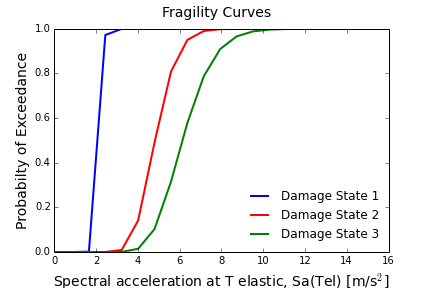
\includegraphics[width=12cm,height=8cm]{./figures/IdealisedCurve.png}
\caption{Display of input Idealised pushover curve.}
\label{fig:expIdealised}
\end{figure}

\begin{figure}[H]
\centering
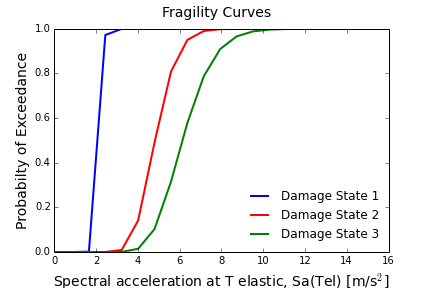
\includegraphics[width=12cm,height=8cm]{./figures/IdealisedCurve.png}
\caption{Display of input pushover curve.}
\label{fig:expPushover}
\end{figure}

In the third step of the code the fragility curves are derived. The parameters extracted are used in the \textit{simplified\_bilinear} or in the \textit{spo2ida} function (according to the analysis method selected with the option \textit{an\_type}) to derive ductility levels $\mu$, median Spectral accelerations $\hat{S}_{a,ds}$ and the total dispersions $\beta_{sc}$ at each damage threshold. These results can be visualised as intermediate outputs during the analysis, as shown below.

\begin{Verbatim}[frame=single, commandchars=\\\{\}, samepage=true]
mu(LS) =  [ 0.73  1.87  2.55]
median IM =  [ 2.11  5.11  6.63]
total dispersion =  [ 0.09  0.32  0.46]
\end{Verbatim}

Medians $\hat{S}_{a,ds}$ and total dispersions $\beta_{sc}$ are converted to logarithmic mean $\mu_{S_a}$ and logarithmic standard deviation $\sigma_{S_a}$, according to the following equations, in order to produce outputs fully compatible with Openquake input models.

\begin{equation}
\mu_{S_a} = \hat{S}_a \frac{\beta_{sc}^2}{2}
\end{equation}
\begin{equation}
\sigma_{S_a} = \sqrt[2]{(\beta_{sc}^2-1) e^{2\ln{ \hat{S}_a}+\beta_{sc}^2}}
\end{equation}

If multiple buildings have been input to derive fragility curves for a class of buildings the Sa at the fundamental period of each building should be converted to a common intensity measure, to be able to combine the different fragility curves. A common intensity measure is selected to be Sa at a period T, which is a weighted average Tav of the individual buildings fundamental period T1. Then each individual fragility needs to be transformed from the original Sa(T1) to the common Sa(T), using a spectrum. FEMA P-695 far field set of 22 accelerograms was used to derive a mean uniform hazard spectrum, and the ratio between the Sa at different periods is used to scale the fragility functions. It can be noted that the actual values of the spectrum are not important, but just the spectral shape. Given the linear transformation, the parameters of the scaled fragility curves of each building are simply:

\begin{equation}
\mu_{iml, blg} = \mu_{iml, blg} S(T_{av})/ S(T_1, blg)
\sigma_{iml, blg} = \sigma_{iml, blg} S(T_{av})/ S(T_1, blg)
\end{equation}

At this stage a single fragility curve is derived 

The logarithmic mean and logarithmic standard deviation are also exported as csv files and the fragility curves can be plotted and saved if the variable \textit{plotflag}[1] has been set to 1 (Figure~\ref{fig:fragility}). These outputs are contained in the folder \textit{outputs}, in the NSP directory.

\begin{figure}[H]
\centering
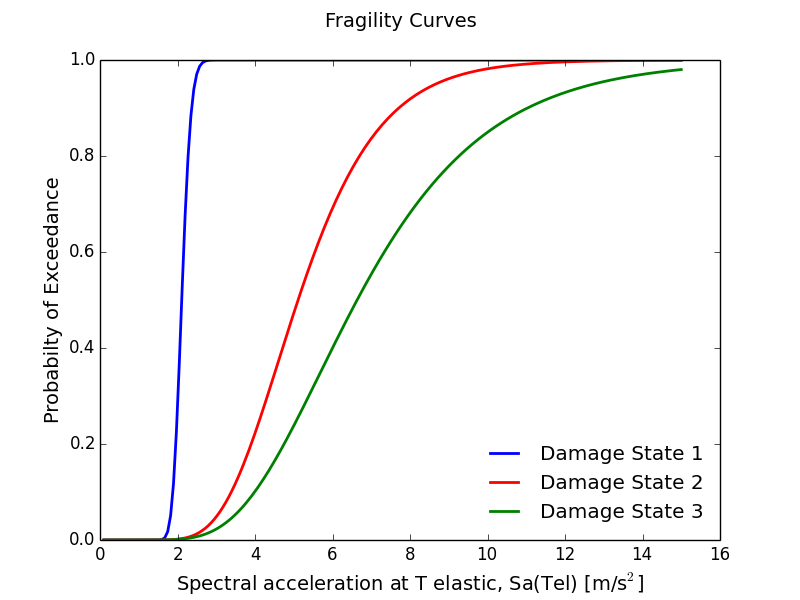
\includegraphics[width=12cm,height=8cm]{./figures/fragility.png}
\caption{fragility curve.}
\label{fig:fragility}
\end{figure}

If the variable \textit{vulnerability} has been set to 1 a vulnerability curve is obtained in the fourth and final step. The derived fragility curves are used in conjunction with the consequence model selected, to get mean values and standard deviations of loss ratios (assuming a lognormal distribution) at the intensity measure levels defined in the options (Section~\ref{par:options}).
As in the case of the fragility curves the results are exported in csv format, and the plot is displayed and saved in png format if the variable \textit{plotflag}[3] is set to 1. Both the csv and the png files can be found in the folder \textit{outputs} in the NSP directory.

\subsection{Procedures for Inelastic Sa estimation}
The workflow presented before works with two different subroutines with respect to the procedure selected to estimate the median $\hat{S}_{a,ds}$ and its dispersion. The inputs to be entered are in some cases different, they are describe in section \ref{subsubsec:CR} and \ref{subsubsec:spo2ida}, along with the step-by-step workflow of each-sub method and the treatment of inter-building uncertainty.

\subsubsection{C$_R$ based procedure}
\label{subsubsec:CR}

The C$_R$ based procedure presented herein, proposed by Vamvatsikos (2014), is applicable to bilinear elasto-plastic capacity curve only. This procedure provides a simple relationship between median damage state threshold, expressed in terms of top displacement $\delta_{roof}$, at each damage state threshold ds, and the corresponding median elastic Spectral displacement value $\hat{S}_{d,ds}(T_1)$.

\begin{equation}
\hat{\delta}_{roof, ds} = C_R S_{d, ds}(T_1) \Gamma_1 \Phi_1
\end{equation}

where $\Gamma_1 \Phi_1$ is the first mode participation factor estimated for the first-mode shape normalised by the roof displacement, and C$_R$ is the inelastic displacement ratio (inelastic over elastic spectral displacement), computed by Ruiz-Garcia and Miranda (2007) for nonlinear SDoF systems having hysteretic behaviour representative of the analysed structure, which is a function of the first-mode period of vibration and the relative lateral strength of the system R. Therefore the median Spectral acceleration at the fundamental period of vibration $\hat{S}_{a,ds}(T_1)$, the seismic intensity measure used in this procedure, turns out to be expressed as a function of the roof displacement according to the following equation:

\begin{equation}
\hat{S}_{a,ds}(T_1) = \frac{4 \pi^2}{\hat{C}_R T^2 \Gamma_1 \Phi_1} \hat{\delta}_{roof, ds}
\label{eq:Sa_RGM}
\end{equation}

Default values of $\hat{C}_R$ parameter estimates are provided by Ruiz-Garcia and Miranda (2007), as result of nonlinear regression analysis of three different measures of central tendency computed from 240 ground motions:

\begin{equation}
\hat{C}_R = 1 + \frac{R - 1}{79.12 T_1 ^{1.98}}
\label{eq:Cr_RGM}
\end{equation}

and values for R are given as:

\begin{equation}
R_{ds} = max(0.425(1 - c + \sqrt{c^2 + 2c(2 \mu_{ds} - 1) + 1}),1)
\label{eq:R_RGM}
\end{equation}

where c = 79.12 T$^{1.98}$, and $\mu_{ds}$ is the ductility at the damage state threshold of interest.

For what concerns the dispersion of $\hat{S}_{a,ds}$, \beta$_{sc}$, the following relationship between S and the median EDP damage threshold $\hat{\theta}$ (Cornell, 2002) is used:

\begin{equation}
\hat{\theta}(s) = a S^b
\end{equation}

so that \beta$_{sc}$ can be easily derived from the dispersion of $\theta$ due to record-to-record variability, $\beta_{\theta d}$, as in the following:

\begin{equation}
\beta_{sc} = \frac{1}{b} \beta_{\theta d}
\label{eq:betaSa_RGM}
\end{equation}

The dispersion of $\theta$ due to record-to-record variability, $\beta_{\theta d}$ can be easily combined with the dispersion of $\theta$ due to uncertainty in the damage state threshold $\beta_{\theta c}$ as shown in the following equation:

\begin{equation}
\beta_{sc} = \frac{1}{b} \sqrt{\beta_{\theta d}^2 + \beta_{\theta c}^2}
\label{eq:betaSc_RGM}
\end{equation}

The dispersion of $\theta$ can be obtained assuming that $d_{roof}$ and $\theta$ are proportional, and they thus share the same dispersion. Moreover the dispersion of $d_{roof}$ is the same as the dispersion of C$_R$, since they are also proportional. Finally $\beta_{\theta d}$ can be computed with the following equation, which represents Ruiz-Garcia and Miranda's (2007) estimate of C$_R$ dispersion:

\begin{equation}
\sigma_{\ln(C_R)} = \sigma_{\ln(d_{roof})} = \beta_{\theta d} =  1.975 [\frac{1}{5.876} + \frac{1}{11.749 (T + 0.1)}] [1- \exp(-0.739 (R - 1))]
\end{equation}

\paragraph{Calculation Steps}
\label{subsec:CalculationSteps}
The medians intensity measure capacity $\hat{S}_{a,ds}$ and corresponding total dispersions $\beta_{sc}$ for different damage thresholds are obtained through the following steps:

\begin{enumerate}
\item Define options and inputs. \textit{an\_type} variable must be set equal to 0. 
	\begin{enumerate}
	\item Dynamic properties of the building (elastic period $T_1$ and modal participation factor $\Gamma_1$ of the first vibration mode), must be input in \textit{building\_parameters.csv}.
	\item Pushover results and Limit States:

If \textit{in\_type} = 0 roof displacement at limit states and idealised pushover curve must be input in \textit{displacement\_profile.csv} and \textit{idealised\_curve} respectively. The only 	parameters needed to describe the idealised pushover curve are the yielding displacement $\delta_y$, the ultimate displacement $\delta_u$ and the yielding force F$_y$.

If \textit{in\_type} = 1 input results from pushover analysis must be input in \textit{displacements\_pushover.csv} and \textit{reactions\_pushover.csv}, and drift limit states in \textit{limits.csv}. The idealised 	pushover curve is then derived in the \textit{idealisation} function, where the idealisation process is conducted according to FEMA-440. The elastic stiffness is defined as the 	tangent stiffness passing through the point of the pushover curve where 60\% of the maximum base shear is reached, and the perfectly plastic branch is set at an height equal to 	the maximum base shear. The yielding point is found as the interception between the elastic and the plastic branch.
	\end{enumerate}
\item Transform the idealised MDoF system to an equivalent SDoF system, using $\Gamma_1$.
\item Define the ductility levels $\mu_{ds}$ corresponding to each damage threshold, expressed in terms of roof displacement.
\item Compute R and C$_R$, using eq. \ref{eq:R_RGM} and \ref{eq:Cr_RGM} respectively.
\item Compute $\hat{S}_{a,ds}$ and the corresponding dispersion  $\beta_{\theta d}$ using eq. \ref{eq:Sa_RGM} and \ref{eq:betaSa_RGM} respectively.
\item Combine $\beta_{\theta d}$ with dispersion due to uncertainty in the model $\beta_{\theta c}$, if different from zero, using eq. \ref{eq:betaSc_RGM} to get the total dispersion $\beta_{sc}$.
\end{enumerate}

\paragraph{Inter-building Uncertainty}
If the vulnerability curve wants to be derived for a class of buildings instead of for a single building the code is able to repeat the process for each single input-building and combine the outputs at the last stage of the results (fragility or vulnerability). 

The fragility results (converted into logarithmic mean and standard deviation of each Limit State) of each building are combined in a single lognormal curve. The parameters of this curve, logarithmic mean and logarithmic standard deviation, are equal to the weighted mean of the single means and the SRSS of the inter-building and intra-building standard deviation, the weighted standard deviation of the single means, and the weighted mean of the single standard deviations, respectively.
The single lognormal fragility curves should not be used to derive a unique vulnerability curve, applying a damage-to-loss function, but only to approximately describe the fragility of a class of buildings, useful for "tagging" purposes for instance.

For the vulnerability curves instead a median loss ratio and the corresponding dispersion for each IML, for each building are derived, assuming a lognormal distribution. A Monte Carlo sampling is performed from these parameters to generate N loss ratios for each building for each IML, finally the mean and standard deviation of the sampled loss ratios is found. These parameters are converted into means and coefficients of variation, which are the parameters consistent with Openquake input model.

In the input files the buildings to be analysed should be inserted as additional lines and weights should be assigned to each building, as in the example below:

\begin{table}[H]
\centering
\begin{tabular}{|c|c|c|c|} \hline
\textbf{n.building} & \textbf{T$_1$} & \textbf{$\Gamma_1$} & \textbf{weights} \\ \hline
1 & 0.32 & 1.23 & 0.2\\ \hline
2 & 0.25 & 1.31 & 0.1 \\ \hline
3 & 0.35 & 1.69 & 0.1 \\ \hline
... & ... & ...& ... \\ \hline
n & 0.41 & 1.54 & 0.2\\ \hline
\end{tabular}
\end{table}

\subsubsection{SPO2IDA based procedure}
\label{subsubsec:spo2ida}
Static PushOver to Incremental Dynamic Analysis (SPO2IDA) is a procedure originally developed by Vamvatsikos and Cornell (2006) and recommended in ATC-58 (FEMA P-58, 2012) that uses empirical relationships from a large database of incremental dynamic analysis results to convert static pushover curves into 16\%, 50\% and 84\% IDA curves, as shown in Figure~\ref{fig:spo2ida}.

\begin{figure}[H]
\centering
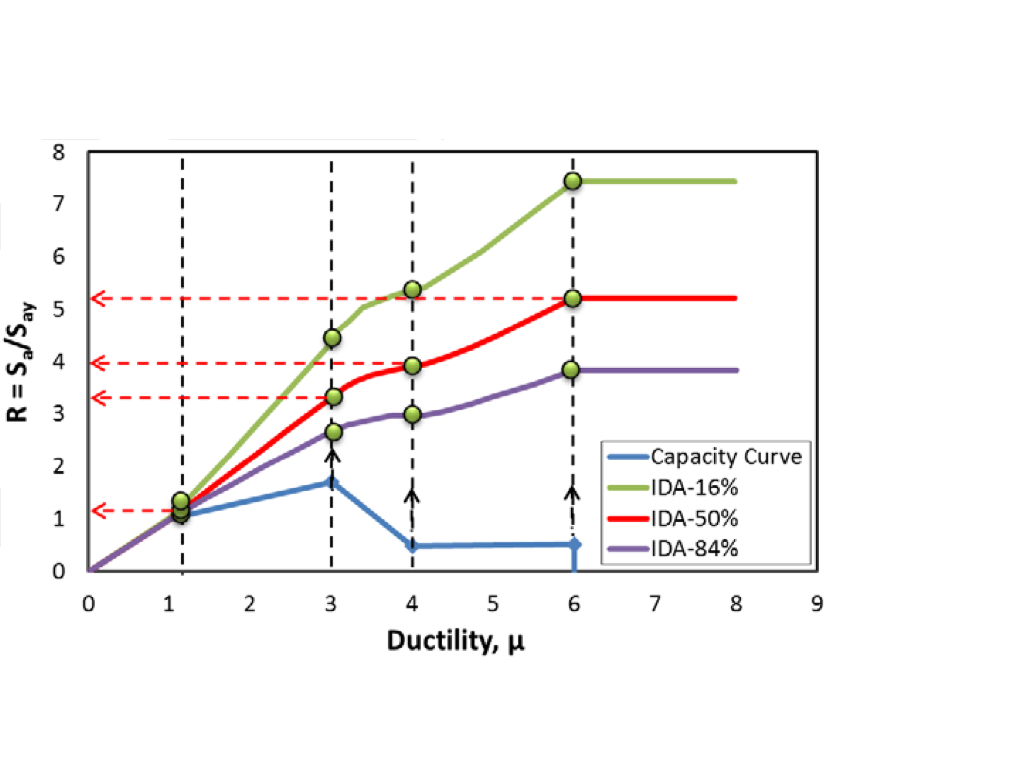
\includegraphics[width=12cm,height=8cm]{./figures/spo2ida.jpg}
\caption{spo2ida tool: IDA curves derived from Pushover curve.}
\label{fig:spo2ida}
\end{figure}

Given the idealised capacity curve the spo2ida tool uses an implicit R - $\mu$ - T relation to correlate nonlinear displacement, expressed in terms of ductility $\mu$ to the corresponding medians capacity in terms of the parameters R. R is the lateral strength ratio, defined as the ratio between the spectral spectral acceleration S$_a$ and the yielding capacity of the system S$_{ay}$. 

Each branch of the capacity curve, hardening, softening and residual plateau, is converted to a corresponding branch of the three ida curves, using the R - $\mu$ - T relation, which is a function of the hardening stiffness, the softening stiffness and the residual force. These parameters are derived from the idealised pushover capacity expressed in $\mu$-R terms, as well as the ductility levels at the onset of each branch. If some of the branches of the pushover curve are missing because of the seismic behaviour of the system, spo2ida can use as input bilinear, trilinear and quadrilinear idealisations.
The result of the spo2ida routine is thus a list of ductility levels and corresponding R values at 50\%, 16\% and 84\% percentiles. The distribution of R values at each ductility level, due to the record-to-record variability, is assumed to be lognormal and it can be easily converted to the dispersion of the lognormal distribution with the following equation:

\begin{equation}
\beta_{R(\mu)} = \frac{\ln R(\mu)_{84\%} - \ln R(\mu)_{16\%}}{2}
\label{eq:betaR}
\end{equation} 

Median R and its dispersion at ductility levels corresponding to the damage thresholds can thus be determined, and $\hat{S}_{a,ds}$ can be easily extracted simply multiplying $R_{50\%}(\mu_{ds})$ by the yielding capacity of the system $S_{ay}$, as shown in the following equation:

\begin{equation}
\hat{S}_{a,ds} = R_{50\%}(\mu_{ds}) S_{ay}
\label{eq:SaR}
\end{equation}
\begin{equation}
S_{ay} = \frac{4 \pi^2 \delta_{roof,y}}{g \Gamma_1 T_1^1}
\end{equation}

Since $\hat{R}$ and $\hat{S}_{a}$ are proportional they share the same dispersion.

\paragraph{Calculation Steps}

\begin{enumerate}
\item Define options and inputs. \textit{An\_type} variable must be set equal to 1. 
\begin{enumerate}
\item Dynamic properties of the building (elastic period and modal participation factor), must be input in \textit{building\_parameters.csv}.

\item Pushover results and Limit States:

If \textit{in\_type} = 0, the roof displacement at each limit state and the idealised pushover curve parameters must be input in \textit{displacement\_profile.csv} and \textit{idealised\_curve} respectively. The 	parameters needed to describe the idealised pushover curve are: yielding displacement d$_y$, displacement at the onset of degradation d$_s$, displacement at the onset of residual force d$_{min}$, ultimate displacement d$_u$, maximum force F$_{max}$, residual force F$_{min}$. These parameters are represented in Figure~\ref{fig:quadrilinear}.

\begin{figure}[H]
\centering
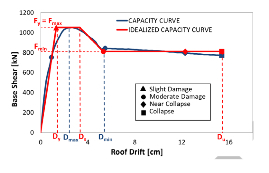
\includegraphics[width=12cm,height=8cm]{./figures/quadrilinear.jpg}
\caption{Idealisation of capacity curve using multilinear elasto-plastic form.}
\label{fig:quadrilinear}
\end{figure}

If \textit{in\_type} = 1 the results from a pushover analysis must be input in \textit{displacements\_pushover.csv} and \textit{reactions\_pushover.csv} and drift limit states in {limits.csv}. The idealised pushover curve is then derived in the \textit{idealisation} function, where the idealisation process is conducted according to the Gem Analytical Vulnerability Guidelines.	\end{enumerate}
\item Transform the idealised MDoF system to an equivalent SDoF system, using \Gamma$_1$, and express SDoF capacity curve in terms of $\mu$-R.
\item Extract from capacity curve variables for spo2ida tool and use them as input to get the 16\%-50\%-84\% ida curves.
\item Define the ductility levels $\mu_{ds}$ corresponding to each damage threshold, and find corresponding R$_{16\%}$-R$_{50\%}$-R$_{84\%}$ in ida outputs.
\item Compute $\hat{S}_{a,ds}$ and the corresponding dispersion $\beta_{\theta d}$ using eq.~\ref{eq:SaR} and eq.~\ref{eq:betaR} respectively.
\item If dispersion due to uncertainty in the model $\beta_{\theta c}$ is different from zero a Monte Carlo sampling needs to be performed. Different values of damage threshold ductilities are sampled from a  lognormal distribution with median the median value of damage threshold ductility and dispersion the input $\beta_{\theta c}$. For each of these ductilities the corresponding R$_{16\%}$-R$_{50\%}$-R$_{84\%}$ are found and converted into $\hat{S}_{a,ds}$ and $\beta_{\theta d}$ according to step 5. N random S$_a$ are sampled from each lognormal distribution with median $\hat{S}_{a,ds}$ and dispersion $\beta_{\theta d}$, corresponding to each sampled ductility. Finally the median and the dispersion of all the sampled S$_a$ are computed, constituting the median $\hat{S}_{a,ds}$ and the total dispersion $\beta_{total}$ considering uncertainty in the damage criteria, for that damage state. The procedure is repeated for each damage state.

\end{enumerate}

\paragraph{Inter-building Uncertainty}
Propagation of uncertainties

\section{Nonlinear Dynamic Method for a class of buildings}
Nonlinear Dynamic Methods are based on the results of many dynamic analyses, which relate the seismic response of a structure, represented by an Engineering Demand Parameter (EDP), like maximum top displacement, maximum inter-storey drift ratio, maximum top drift etc., to the Intensity Measure Level of the input accelerograms. 
Many methods exists in literature to perform a series of dynamic analysis and to post-process the results in order to derive fragility curves. Some of them treat a single building to estimate directly the median seismic intensity value corresponding to the attainment of different damage state threshold (limit state), and the corresponding dispersion (Vamvatsikos and Cornell, 2002, Ellingwood and Kinali, 2009). Others treat a class of buildings, and lead to the evaluation of the probabilities of different damage states for a series of IMLs and thus to the set up of a damage probability matrix (Singhal and Kiremidjian, 1996, Silva et al., 2013).

The last approach have been followed in the current implementation: the results of a set of dynamic analysis, in terms of EDP and corresponding IML for each structure of the building class, are compared with the limit state displacements and a global damage state is assigned to each structure. Thus, for each record, the number of frames in each damage state is obtained. This distribution of buildings in each damage state can be organised in a damage probability matrix, with a number of rows equal to the number of ground motion records and a number of columns equal to the number of damage states. Regression analysis (maximum likelihood method) is then applied to this data to fit a lognormal curve for each limit state (leading to a fragility curve), where the record-to-record variability is accounted for by the use of many ground motion records, and the inter-building variability is accounted for subjecting to the same set of accelerograms hundreds of structures representing the entire building class.

The last approach have been followed in the current implementation. The script takes care only of the post-processing part, therefore the results of a set of dynamic analyses previously run have to be input to start the process. A list of intensity measure associated to each accelerogram, and corresponding EDP for each structure of the building class can be input, along with the set of limit states expressed in terms of the same EDP. The EDPS resulting from the dynamic analyses are compared with the limit state displacements and a global damage state is assigned to each structure. Thus, for each record, the number of frames in each damage state is obtained. This distribution of buildings in each damage state can be organised in a damage probability matrix, with a number of rows equal to the number of ground motion records and a number of columns equal to the number of damage states plus one: in the first position of each row the IML of each record is located, followed by the percentage of buildings in each damage state. Alternatively a damage probability matrix can be computed directly using as input a damage count matrix, which corresponds to a damage probability matrix, where the probabilities of each damage state are substituted by the count of buildings in that damage state. Regression analysis (maximum likelihood method) is then applied to this data to fit a lognormal curve for each limit state, leading to fragility curves. These functions have the advantage of accounting for the record-to-record variability by the use of many ground motion records, and the inter-building variability subjecting to the same set of accelerograms hundreds of structures representing the entire building class.

\subsection{Method Workflow}
To get started with the Nonlinear Dynamic Method a command line text editor should be used to enter manually the folder location where the RMTK has been saved. The user should add the path /RMTK/Vulnerability/NDP, where the Nonlinear Dynamic Method script (NDM.py) is located, as shown in the example below:

\begin{Verbatim}[frame=single, commandchars=\\\{\}, samepage=true]
\$ cd path/to/rmtk/folder/RMTK/Vulnerability/NDP
\end{Verbatim}

From the text editor iPython browser page can be opened with the following command line:

\begin{Verbatim}[frame=single, commandchars=\\\{\}, samepage=true]
\$ ipython-2.7 notebook --pylab=inline
\end{Verbatim}

Once the iPython page is opened on the browser, the python scripts contained in the NDP directory will be visible. The file \textit{NDM.ipynb} should be selected to start the calculations.
In the first step of the code the initial options and the inputs must be defined, as described in the following section.

\subsubsection{Options}
In the Options the user has to define first of all the type of inputs at disposal, setting the variable \textit{in\_ type}, choosing between:

\begin{Verbatim}[frame=single, commandchars=\\\{\}, samepage=true]
in\_type = 0 # input is a Damage Count Matrix with number of buildings in each damage state
in\_type = 1# input is a matrix with engineering demand parameter corresponding to IML of each dynamic analysis
\end{Verbatim}

The variable \textit{vulnerability} instead gives the opportunity to stop the process at the derivation of the fragility curves, or to go all the way up to the vulnerability curve definition applying damage-to-loss functions.

\begin{Verbatim}[frame=single, commandchars=\\\{\}, samepage=true]
vulnerability = 0 # stop at fragility curves
vulnerability = 1 # derive vulnerability curve
\end{Verbatim}

The variable \textit{iml} is a numpy array that identifies the intensity measure levels for which loss ratios are computed and provided in the vulnerability curve.

\begin{Verbatim}[frame=single, commandchars=\\\{\}, samepage=true]
iml = np.linspace(0.1,15,100)
\end{Verbatim}

The variable \textit{plotflag} allows or inhibits the displaying of plots. It is a list composed of 2 integers, each one controlling a different plot: fragility curves and vulnerability curve. Each integer can take as value either zero or one, whether the corresponding graph has to be displayed or not:

\begin{Verbatim}[frame=single, commandchars=\\\{\}, samepage=true]
plotflag = [1, 1] # plot all the graphs
plotflag = [0, 0] # do not plot any graph
\end{Verbatim}

The following variables set some of the characteristics of the plots:
\begin{itemize}
\item linew: integer for defining lines width.
\item fontsize : fontsize used for labels, graphs etc.
\end{itemize}

\subsubsection{Inputs}
The inputs must be formatted as comma-separated value files (.csv), and saved in the folder \textit{input}, contained in the NDP directory. If any other environment different from Windows is used make sure that the ”comma separated format Windows” is selected as saving option when creating the input files. As previously mentioned two types of input can be entered, whether the results the set of dynamic analyses performed have already been organised in a damage probability matrix for or not. In the former case the variable \textit{in\_type} should be set to 0 and the damage count matrix should be input in the csv file \textit{dcm.csv}. The first two columns refer to the number of record and the corresponding intensity measure level, the following columns report the number of buildings in each damage state, as shown in the following table:

\begin{table}[H]
\centering
\begin{tabular}{|c|c|c|c|c|} \hline
\textbf{n.records} & \textbf{Intensity Measure Level} & \textbf{DS$_0$} & \textbf{DS$_1$} & \textbf{DS$_2$} \\ \hline
1 & 49.852 &	30 &	16 &	54\\ \hline
2 & 47.056 &	54 &	15 &	31\\ \hline
3 & 33.012 &	59 &	10 &	31\\ \hline
4 & 82.125 &	24 &	26 &	50\\ \hline
... & ... & ... & ... & ... \\ \hline
5 & 37.499 &	58 &	5 &	37\\ \hline
\end{tabular}
\end{table}

In the latter case each building subjected to an accelerogram provide as result an EDP which is stored in the columns of a matrix following the number of record and the corresponding IML \textit{edp.csv}

\begin{table}[H]
\centering
\begin{tabular}{|c|c|c|c|c|c|} \hline
\textbf{n.records} & \textbf{IML} & \textbf{edp$_{blg,1}$} & \textbf{edp$_{blg,2}$} & \textbf{...} & \textbf{edp$_{blg,n}$} \\ \hline
1 &	69.209 &	-0.00069 &	0.00031 & ... &	0.00131\\ \hline
2 &	75.470 &	0.00102 & 	0.00202 & ... &	0.00302\\ \hline
3 &	62.233 &	-0.00090 &	0.00010 & ... &	0.00110\\ \hline
4 &	168.47 &	-0.00246 &	-0.00146 & ... &	-0.00046\\ \hline
5 &	67.612 &	0.00095 & 	0.00195 & ... &	0.00295\\ \hline
... & ... & ... & ... & ... & ...\\ \hline
n &	34.484 &	0.00036 & 	0.00136 & ... & 	0.00236\\ \hline
\end{tabular}
\end{table}

limits.csv
\begin{table}[H]
\centering
\begin{tabular}{|c|c|c|c|c|} \hline
\textbf{n.building} & \textbf{LS$_1$} & \textbf{LS$_2$} & \textbf{LS$_3$} & \textbf{LS$_4$} \\ \hline
1 & 0.003 &	0.010 &	0.025 &	0.0337\\ \hline
2 & 0.004 &	0.015 &	0.020 &	0.035\\ \hline
3 & 0.002 &	0.019 &	0.027 &	0.032\\ \hline
... & ... & ... & ... & ...\\ \hline
n & 0.0024 &	0.016 &	0.025 &	0.03\\ \hline
\end{tabular}
\end{table}

\subsubsection{Calculations}
# Read data from csv input file and get: damage count matrix, total number of buildings analysed, Intensity Measures of each record, number of Limit States
#Transform Damage Count Matrix into matrix of probability of exceedance each damage
# Fit number of buildings exceeding each level of damage with Maximum Likelihood regression method
# Derive vulnerability curves from damage-to-loss ratios

